%
% File acl2018.tex
%
%% Based on the style files for ACL-2017, with some changes, which were, in turn,
%% Based on the style files for ACL-2015, with some improvements
%%  taken from the NAACL-2016 style
%% Based on the style files for ACL-2014, which were, in turn,
%% based on ACL-2013, ACL-2012, ACL-2011, ACL-2010, ACL-IJCNLP-2009,
%% EACL-2009, IJCNLP-2008...
%% Based on the style files for EACL 2006 by 
%%e.agirre@ehu.es or Sergi.Balari@uab.es
%% and that of ACL 08 by Joakim Nivre and Noah Smith

\documentclass[11pt,a4paper]{article}
\usepackage[hyperref]{acl2018}
\usepackage{times}
\usepackage{latexsym}
\usepackage{graphicx}
\usepackage{float}
\usepackage{url}

\aclfinalcopy % Uncomment this line for the final submission
%\def\aclpaperid{***} %  Enter the acl Paper ID here

%\setlength\titlebox{5cm}
% You can expand the titlebox if you need extra space
% to show all the authors. Please do not make the titlebox
% smaller than 5cm (the original size); we will check this
% in the camera-ready version and ask you to change it back.

\newcommand\BibTeX{B{\sc ib}\TeX}

\title{Language Understanding System: Mid-term Project}

\author{Montagner Andrea \\
  {\tt andrea.montagner@studenti.unitn.it}}

\date{\today}

\begin{document}
\maketitle
\begin{abstract}
The aim of this project is to develop a Spoken Language Understanding module for the Movie Domain capable of performing PoS tagging. In order to achieve this goal a language model is firstly created and then trained to predict unseen utterances from a testing pool of data. In the following sections multiple approaches with respective solutions are presented, each one evaluated in term of accuracy, precision, recall and f1 score. Finally these results are compared to each other in order to determine the best approach to this problem.
\end{abstract}

\section{Introduction}

A Concept Tagger is a module which is capable of assigning a concept, in this case a tag, to words belonging to a sentence. This operation, though, requires the presence of a dataset composed by couples (words, tag) large enough to have a sufficient number of utterances to perform both the training and testing phase.\\
In particular, the material that was provided for this project was:
\begin{itemize}
	\item A train dataset, both for the Movie Domain and for the additional features,
	\item A test dataset, both for the Movie Domain and for the additional features,
	\item A Perl script, {\tt "conlleval.pl"}, to evaluate the performances in terms of accuracy, precision, recall and f1 score.
\end{itemize}


\section{Data Analysis}
\label{sec:datanalysis}

The provided dataset is the Microsoft NL-SPARQL dataset and it was already split into two parts: one for training and one for testing. In addition, each of these groups of data was divided into main data for the Movie Domain and additional features. The latter contains lemmas and PoS (Part of Speech) tags for each word.\\ 
To summarize, what was given were four files:
\begin{itemize}
	\item \textbf{NL-SPARQL.train.data} containing a two columns set of data, tab separated, where the first column represent the words and the second tags,
	\item \textbf{NL-SPARQL.train.feats.txt} containing a three columns set of data, tab separated, where the first column represent words, the second PoS tags and the third lemmas,
	\item \textbf{NL-SPARQL.test.data} containing a two columns set of data, tab separated, where the first column represent words and the second tags,
	\item \textbf{NL-SPARQL.test.feats.txt} containing a three columns set of data, tab separated, where the first column represent the words, the second tags and the third lemmas.
\end{itemize}

In these files, each line contains a word (with the respective tag/lemma) of a sentence and the end of each sentence is marked with an empty line as delimiter. (\ref{firsttab}).\\

\begin{table}[]
\centering
\label{firsttab}
\begin{tabular}{|l|l|}
\hline
\begin{tabular}[c]{@{}l@{}}{\tt who}\\ {\tt plays}\\ {\tt luke}\\ {\tt on}\\ {\tt star}\\ {\tt wars}\\ {\tt new}\\ {\tt hope}\\ \\ {\tt show}\\ {\tt credits}\\ {\tt for}\\ {\tt the} \\ {\tt godfather}\end{tabular} & \begin{tabular}[c]{@{}l@{}}{\tt O}\\ {\tt O}\\ {\tt B-character.name}\\ {\tt O}\\ {\tt B-movie.name}\\ {\tt I-movie.name}\\ {\tt I-movie.name}\\ {\tt I-movie.name}\\ \\ {\tt O}\\ {\tt O}\\ {\tt O}\\ {\tt B-movie.name}\\ {\tt I-movie.name}\end{tabular} \\ \hline
\end{tabular}
\caption{An example of the structure of train data}
\end{table}

\begin{table}[h]
\centering
\label{firsttab}
\begin{tabular}{|l|l|l|}
\hline
\begin{tabular}[c]{@{}l@{}}{\tt who}\\ {\tt plays}\\ {\tt luke}\\ {\tt on}\\ {\tt star}\\ {\tt wars}\\ {\tt new}\\ {\tt hope}\\ \\ {\tt show}\\ {\tt credits}\\ {\tt for}\\ {\tt the} \\ {\tt godfather}\end{tabular} & \begin{tabular}[c]{@{}l@{}}{\tt WP}\\ {\tt VVZ}\\ {\tt NN}\\ {\tt IN}\\ {\tt NN}\\ {\tt NNS}\\ {\tt JJ}\\ {\tt NN}\\ \\ {\tt NN}\\ {\tt NNS}\\ {\tt IN}\\ {\tt DT}\\ {\tt NN}\end{tabular} & \begin{tabular}[c]{@{}l@{}}{\tt who}\\ {\tt play}\\ {\tt luke}\\ {\tt on}\\ {\tt star}\\ {\tt war}\\ {\tt new}\\ {\tt hope}\\ \\ {\tt show}\\ {\tt credit}\\ {\tt for}\\ {\tt the} \\ {\tt godfather}\end{tabular} \\ \hline
\end{tabular}
\caption{An example of the structure of feats data}
\end{table}

\subsection{Data Distribution}

A deeper analysis, instead, shows how both IOBs and words distributions follow an empirical statistical law, called \textit{Zipf's Law}, for which the frequency of a word is inversely proportional to its rank in the frequency table.\\

The next two subsections will illustrate a more detailed analysis of the data, focusing individually first on IOBs and then on words.

\subsubsection{IOB Definition \& Distribution}
 
 Concept Tags are represented using an \textit{IOB notation}, which is a common tagging format when dealing with chunking tasks like identifying different parts of a string. \\
 The used prefixes are:
 \begin{itemize}
 	\item \textbf{B} - Beginning of a span
 	\item \textbf{I} - Inside of a span
 	\item \textbf{E} - End of a span
 	\item \textbf{O} - Outside of a span
 \end{itemize}
 
As long as IOBs distributions is concerned, the analysis mirrors the prediction and outputs as the most frequent tag {\tt movie.domain}, divided in {\tt I.movie.domain} and {\tt B.movie.domain}.\\

In this analysis the tag {\tt "O"} is not taken into consideration because it can be considered a "stop-word" for tags.
 
\begin{figure}[H]
	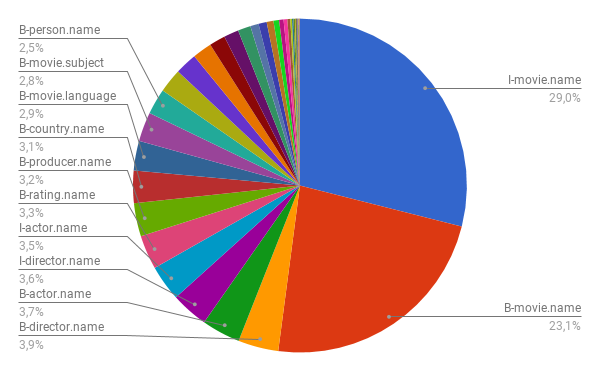
\includegraphics[scale=.35]{img/IOB_chart_noO.png}
	\label{fig:f1res}
\end{figure}

\subsubsection{Words Distribution}

Almost all of most frequent words are identified as stop words, like {\tt the} ($1337$), {\tt of} ($607$), {\tt in} ($582$). Nonetheless there are exceptions, like {\tt movies} ($1126$) and {\tt movie} ($564$), which are relevant to understand the topic of the considered dataset.

\begin{figure}[H]
	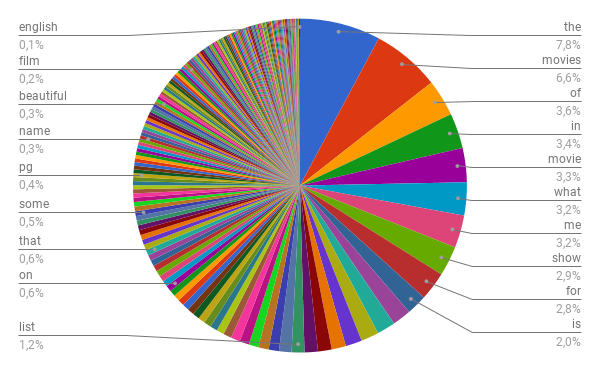
\includegraphics[scale=.35]{img/Word_chart.png}
	\label{fig:f1res}
\end{figure}

%\subsection{Additional Features}
%\label{subsect:addfeat}
%
%Additional feature files contain labels and PoS tags for each word, both training and testing. At the beginning, the idea was that these features could have allowed a better training and consequently better evaluations but after some attempts the results were actually worse.
%
%The formulas for the probability used when dealing taking into account additional features are:\\
%
%	$\frac{P(word, lemma, IOB)}{P(IOB)}$ if using lemmas \\\\
%	$\frac{P(word, PoS_{tag}, IOB)}{P(IOB)}$ if using PoSTags



%
%\begin{table*}
%\centering
%\begin{tabular}{lll}
%  output & natbib & previous ACL style files\\
%  \hline
%  \citep{Gusfield:97} & \verb|\citep| & \verb|\cite| \\
%  \citet{Gusfield:97} & \verb|\citet| & \verb|\newcite| \\
%  \citeyearpar{Gusfield:97} & \verb|\citeyearpar| & \verb|\shortcite| \\
%\end{tabular}
%\caption{Citation commands supported by the style file.
%  The citation style is based on the natbib package and
%  supports all natbib citation commands.
%  It also supports commands defined in previous ACL style files
%  for compatibility.
%  }
%\end{table*}
\section{Tools and Implementation}

The whole project was developed using Bash and Python (v2.7) as programming languages. In addition, two external tools were provided, in order to perform specific actions (\textit{i.e.} creation of the transducer and of the language model). This tools are:
\begin{itemize}
	\item \textbf{OpenFST} library \cite{fst}
	\item \textbf{OpenGrm} Ngrm library \cite{ngr}
\end{itemize}

All tried training algorithms are performed for $5$ different ngram order ($1$ to $5$) and for each smoothing method offered by OpenFST, namely \textit{absolute}, \textit{katz}, \textit{kneser\_ney}, \textit{presmoothed}, \textit{unsmoothed}, \textit{witten\_bell}. The only method which is not used is \textit{katz\_frac}, because it is not working.\\

The case of a transducer words to IOBs will be considered as baseline method for this project and its results compared to other approaches to evaluate which one best suites the problem.

\subsection{Baseline method}

This first attempt takes into consideration only the basic data files, containing words and concepts. The idea is to see concepts as classes to be predicted and train the model using the probability of words given concepts. For this reason, the best approach seemed to be the \textit{Bayesian Decision Rule} to compute the Maximum Likelihood estimation:
\begin{equation}
\label{probw2iob}
	P(word\,|\,IOB)=\frac{C(word,\,IOB)}{C(IOB)}
\end{equation}
	
	Where $C(word,\,IOB)$ is the number of occurrences of the couple $(word, IOB)$, and $C(IOB)$ is the number of total occurrences of that IOB. However, since the final output will be an automaton, probabilities are not the best value to estimate moves between states. For this reason, instead of the Maximum Likelihood, it is used its negative logarithm:
	
	\[Cost(word\,|\,IOB)=-log(P(word\,|\,IOB)) \]
	
	Unknown words are handled assigning to all concepts the same probability to generate them. In this way, the costs become:

	\[Cost(<unk>|\,IOB)=-log(\frac{1}{\#IOBs})) \]	

\subsection{Other approaches: different training methods}
\label{ssec:otherapp}



\subsubsection{Cut-off}

The first idea to improve the accuracy of the prediction was the insertion of a \textit{frequency cut-off} value on words not to take into consideration all those words (with their respective IOB) whose frequency lay below a certain threshold (empirically set to $50$). With this add-on, each method (both the baseline and the ones that will be explained later on) could be tested with or without this threshold in order to have a more accurate idea on how evaluation changes.\\

Interesting to report is how unknown words are handled in this case. Unlike the baseline solution, assigning the same probability to all the concepts would not be correct. The reason is that the number of times an IOB is deleted is known in advance and this gives the possibility to perform a more accurate computation of the probability, which becomes:
\begin{enumerate}
	\item Compute the new probability $P(word_a\,|\,IOB)$ as before
	\item Compute the difference between $P(word\,|\,IOB)$ before and after the cutoff:
		\begin{equation}
			\resizebox{.75\hsize}{!}{$ProbCF=P(word_b\,|\,IOB)\,-\,P(word_a\,|\,IOB)$}
		\end{equation}
	\item Add $ProbCF$ to the previous probability for \textit{$<unk>$}:
		\begin{equation}
			\resizebox{.75\hsize}{!}{$P(<unk>|\,IOB)=\frac{1}{\#IOBs}*ProbCF$}
		\end{equation}
		
		In this way probability of unknown words given a specific IOB increase depending on how many times that IOB is deleted because of the cut-off.
\end{enumerate}

\subsubsection{Lemma2IOB}

The second attempt for trying to boost the performances was using lemmas instead of words. Lemmas can be found in the additional features files (\ref{sec:datanalysis}). The Maximum Likelihood is computed as follow:

\begin{equation}
\label{probl2iob}
	P(lemma\,|\,IOB)=\frac{C(lemma,\,IOB)}{C(IOB)}
\end{equation}

As can be seen, this method is very similar to the baseline, just replacing words with lemmas. Probabilities are then transformed into costs as before (negative log likelihood), and unknown words are handled with the same policy. 

\subsubsection{O-removal}

Another attempt to enhance the performances was trying to remove the {\tt "O"} tag from the set. The reason is that it brings no valuable information (as stated before, can be seen as a "stop word" for tags) since most of words are tagged as "out of span". The idea was to replace it with the word itself (\textit{i.e.} (show, O) becomes (show, O-show)). With this little trick the model gains a lot of more information about other tags allowing a better training phase and consequently better results in the prediction.\\

This method was applied only to the baseline Word to IOB solution. The structure is the same as before, both for probabilities computation and handling of unknown words. The only difference is a modified training set where there are no {\tt "O"} tags

\begin{figure*}[h]
	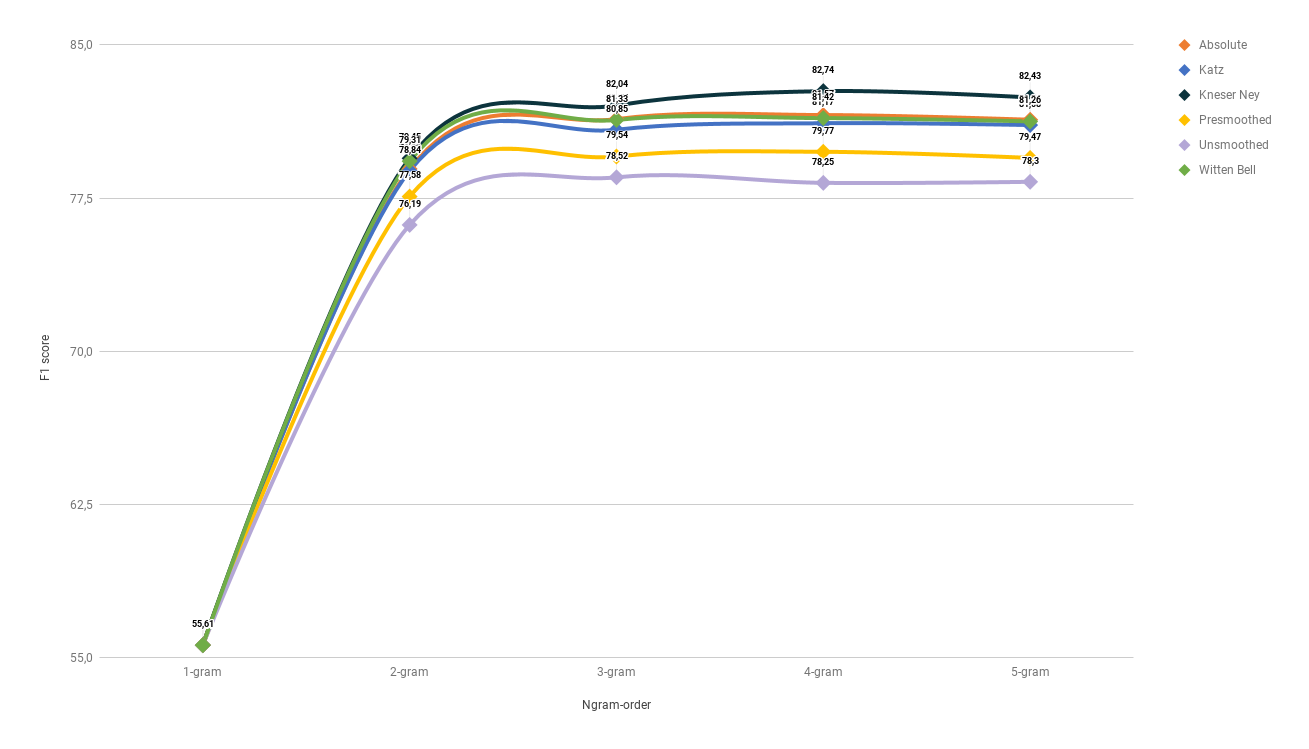
\includegraphics[width=\textwidth]{img/chart.png}
	\caption{F1 scores for the Word to Concept method without 'O'}
\end{figure*}

\section{Evaluations Analysis}

Evaluations in performed by a Pearl script, {\tt conlleval.pl}, which evaluates four different scores: \textit{Accuracy}, \textit{Precision}, \textit{Recall}, \textit{F1}.

\[Accuracy=\frac{TP\,+\,TN}{TP\,+\,TN\,+\,FP\,+\,FN}\]
\[Precision=\frac{TP}{TP\,+\,FP}\]
\[Recall=\frac{TP}{TP\,+\,FN}\]
\[F1\footnote{This is a simplified version of the F1 Score formula where $\beta=1$, the complete formulation is:\\\\ $(1*\beta^{2})\frac{Precision\,*\,Recall}{(\beta^{2}*Precision)\,+\,Recall}$}=\frac{Precision\,*\,Recall}{Precision\,+\,Recall}\]

\subsection{Word2IOB Evaluation}

Analyzing the output of the evaluation script for the baseline approach, best performances are:
\begin{itemize}
	\item Accuracy: $92,68$
	\item Precision: $78,51$
	\item Recall: $74,34$
	\item F1: $76,37$
\end{itemize}

and correspond to the \textit{witten\_bell} method with \textit{bigrams}. Similar values are found using \textit{bigrams} with the \textit{kneser
\_ney} method.  These values drop drastically when considering unigrams, while float around the same value for ngram order from $2$ to $5$. More in general, it is not the best approach to solve this problem, there are solutions which present better performances.

\subsection{Cut-off}

The insertion of a cut-off value as threshold was an experiment that did not give the expected results. After the analysis of the results on the baseline solution the decision was to not apply it to the other approaches. Performances drop a lot throughout all methods, independently from which ngram order is used. Just as a report, best performances are:
\begin{itemize}
	\item Accuracy: $71,73$
	\item Precision: $731,91$
	\item Recall: $32,391$
	\item F1: $32,40$
\end{itemize}
and correspond to the \textit{unsmoothed} method with \textit{4-grams}.

\subsection{Lemma2IOB Evaluation}

Also this approach, like the use of a cut-off frequency, does not give good results as output. Very likely the reason lay in how the probability is computed, which may not be the best way. Also here, just as a report, best performances are:
\begin{itemize}
	\item Accuracy: $89,59$
	\item Precision: $71,17$
	\item Recall: $60,86$
	\item F1: $65,61$
\end{itemize}
and correspond to the \textit{witten\_bell} method with \textit{bigrams}.


\subsection{Word2IOB without 'O'}

This is the last approach that has been tried and the one who actually gives the best results of all. Performances, with this method, rise of almost 20\% as far as F1 score is concerned. Best values are found for \textit{Kneser Ney} method using 4-grams. More in details, values are:
\begin{itemize}
	\item Accuracy: $94,96$
	\item Precision: $82,44$
	\item Recall: $83,04$
	\item F1: $82,74$
\end{itemize}

Comparing these values to the ones of the baseline method, it can be seen that the worst value of this approach, that is $76,19$ using \textit{Unsmoothed} with bigrams (unigram values are not taken into consideration due to the fact that are too out of range to be comparable) are very similar to the best results of the baseline solution. As already mentioned, the reason of this sharp raise is that, increasing the generalization with the removal of the {\tt "O"} tag, the system gain the capability learning more information about other concepts.\\
Figure 1 shows the complete evaluation of these results, for all considered smoothing methods, each of them with ngram order from $1$ to $5$.

\section{Conclusions}

In this project different methods develop a Spoken Language Understanding module for the Movie Domain are presented. Each of them has been tested and compared to the one taken as 'Baseline Solution', namely the Word2IOB approach. After a pre-processing phase where data have been organized so to be able to be used in he training, model has been first trained and then tested on different datasets. As mentioned before, best solution are given from the Word2IOB without {\tt "O"} approach, it allowing more generalization of the tags. In future, more approach could be performed, using also PoS Tags or combining words with lemmas. The issue would be to individuate a good formulation of the computation of the probability, which could maybe lead to better performances.


% include your own bib file like this:
%\bibliographystyle{acl}
%\bibliography{acl2018}
\bibliography{acl2018}
\bibliographystyle{acl_natbib}

\end{document}
